\documentclass{article}
\usepackage{graphicx} % Required for inserting images
\usepackage{authblk}
\usepackage{amsmath}
\usepackage{stmaryrd}
\usepackage{amssymb}
\usepackage{xcolor}
\usepackage{multirow}
\usepackage{booktabs}

\usepackage{tikz}
\usepackage{tikz-3dplot}
\usetikzlibrary{arrows.meta, decorations.pathmorphing, backgrounds, calc, patterns, shapes.geometric}

\def\correspondingauthor{\footnote{Corresponding author: louis.libat2@univ-eiffel.fr}}

\title{Geometric Strategies for Sharp-Interface Front-Tracking Methods}
\author[1]{Thomas Sobre}
\author[1]{Louis Libat \correspondingauthor}
\author[1]{Can Selçuk}
\author[1]{Eric Chénier}
\author[1]{Vincent Le Chenadec}
\affil[1]{MSME, Université Gustave Eiffel, UMR CNRS 8208, Marne-la-Vallée, 77454, France}
\date{\today}

\begin{document}

\maketitle

\begin{abstract}
    xxx
\end{abstract}

\section{Notes}
- Pure front-tracking, no coupling to a solver. 
- Bibliography, litterature review of current Front tracking method, markers maintenance, hygiene,
- The differents front tracking problems (merging, breakup, redistribution, insertion, ....)
- Algorithms
- why only normal component ? Because fundamentally, front is moving with front velocity, which is normal to the front. 
- Only normal component of velocity, no tangential redistribution => What's going one ? Add redistribution => better ?
- Numerical Tests
- DEC, DDG
- References

\section{Introduction}

\cite{koffi_bi_accuracy_2022}

\section{Continuum Sharp interface formulation}
\label{sec:governing}

Let $\Omega\subset\mathbb{R}^d$ be a fixed domain, with $d\in\{2,3\}$, and let $\Gamma(t)\subset\Omega$ be a moving interface separating two distinct phases.
The interface $\Gamma(t)$ is a codimension-one manifold, that is, a curve when $d=2$ and a surface when $d=3$.
The interface evolves according to a normal velocity field $V_n$ defined on $\Gamma(t)$, which may depend on the local geometry of the front and on physical fields such as pressure, temperature, or concentration.
The governing equation for the interface motion is therefore
\begin{equation}
\frac{\partial \Gamma}{\partial t} = V_n n, 
\label{eq:interface_motion}
\end{equation}
where $n$ is the unit normal vector field on $\Gamma(t)$ pointing from one phase to the other.
$V_n$ may include contributions from curvature, external forces, or other physical effects, depending on the specific problem under consideration. 





\section{Lagrangian front-tracking representation and intrinsic geometric operators}
\label{sec:front_tracking}

In the present work, the moving sharp interface is represented explicitly by a
Lagrangian front mesh. The front is the primary geometric unknown: all normals,
curvatures, intrinsic differential operators, are constructed from this mesh.
The purpose of this section is therefore twofold:
(i) to define the minimal discrete data required to represent the interface in
two and three space dimensions, and
(ii) to introduce the intrinsic geometric and differential operators that can be
constructed directly on this front.

The front-tracking representation described here concerns codimension-one
interfaces in $d\in\{2,3\}$, namely polygonal curves in two dimensions and
triangulated surfaces in three dimensions.

At time $t$, the discrete interface is denoted by $\Gamma_h(t)$, and its vertex
positions are gathered in the vector
\begin{equation}
X(t) = \{x_a(t)\}_{a=1}^{N_v}.
\label{eq:front_vertices}
\end{equation}
Here $h$ denotes the characteristic front-mesh size, and $N_v$ is the number of
front vertices. The notation emphasizes that $\Gamma_h(t)$ is a discrete approximation
of the smooth interface $\Gamma(t)$ introduced in Section~\ref{sec:governing}.
For simplicity, the explicit dependence on time is omitted below whenever no ambiguity arises.

\subsection{Discrete front mesh}
\label{subsec:front_mesh}

The discrete front representation depends on the ambient space dimension.

\paragraph{Two-dimensional front.}
When $d=2$, the interface is represented by a polygonal curve
\begin{equation}
\Gamma_h = (V_h,E_h),
\end{equation}
where $V_h=\{x_a\}_{a=1}^{N_v}\subset\mathbb{R}^2$ is the set of front vertices
and $E_h=\{e\}_{e=1}^{N_e}$ is the set of oriented edges.
Each edge $e=(i,j)$ connects two consecutive vertices and is oriented from $x_i$
to $x_j$.

\paragraph{Three-dimensional front.}
When $d=3$, the interface is represented by a triangulated surface
\begin{equation}
\Gamma_h = (V_h,F_h),
\end{equation}
where $V_h=\{x_a\}_{a=1}^{N_v}\subset\mathbb{R}^3$ is the set of front vertices
and $F_h=\{f\}_{f=1}^{N_f}$ is the set of oriented triangular faces.
Each face $f=(i,j,k)$ is oriented consistently with the global orientation of the surface.

In both cases, the front mesh is fully determined by the vertex coordinates $x_a$, 
the mesh connectivity and a consistent orientation.
No additional geometric unknown is introduced at this stage.
All normals, curvatures, and intrinsic operators are reconstructed from these quantities.

Unless stated otherwise, $\Gamma_h$ is assumed to be an orientable manifold
mesh, closed for embedded internal interfaces and possibly with boundary for
open-front test cases. In particular, the mesh connectivity is assumed to be
compatible with a globally consistent orientation.

\subsection{Topology, orientation, and adjacency}
\label{subsec:front_topology}

A front mesh is not merely a collection of points embedded in physical space:
it also carries a combinatorial structure that determines local neighborhoods,
orientation signs, and discrete differential stencils.

For a curve mesh, the relevant topological information is the vertex-edge incidence.
For a triangulated surface, one additionally needs:
\begin{itemize}
    \item the set of unique edges,
    \item the vertex-edge adjacency,
    \item the vertex-face adjacency,
    \item the edge-face adjacency,
    \item the orientation of each face relative to its boundary edges.
\end{itemize}

This structure is encoded by incidence operators.
For both curves and surfaces, the discrete exterior derivative from vertices to edges is
\begin{equation}
d_0 : C^0(\Gamma_h) \longrightarrow C^1(\Gamma_h),
\end{equation}
where $C^0(\Gamma_h)$ denotes vertex-based scalar fields and $C^1(\Gamma_h)$ denotes
oriented edge-based quantities. For a scalar field $u_h=\{u_a\}_{a=1}^{N_v}$,
\begin{equation}
(d_0 u_h)_e = u_j-u_i,
\qquad e=(i,j).
\label{eq:d0_def}
\end{equation}

In three dimensions, one further introduces the discrete exterior derivative from
edges to faces,
\begin{equation}
d_1 : C^1(\Gamma_h) \longrightarrow C^2(\Gamma_h),
\end{equation}
where $C^2(\Gamma_h)$ denotes face-based quantities.
For a consistently oriented triangulated surface, the identity
\begin{equation}
d_1 d_0 = 0
\label{eq:exact_sequence}
\end{equation}
holds exactly at the discrete level.

This topological layer is essential for the construction of intrinsic geometric
operators on the front. It also provides natural consistency checks, such as
closedness, manifoldness, and global orientation coherence.

\subsection{Minimal geometric data}
\label{subsec:front_geometry}



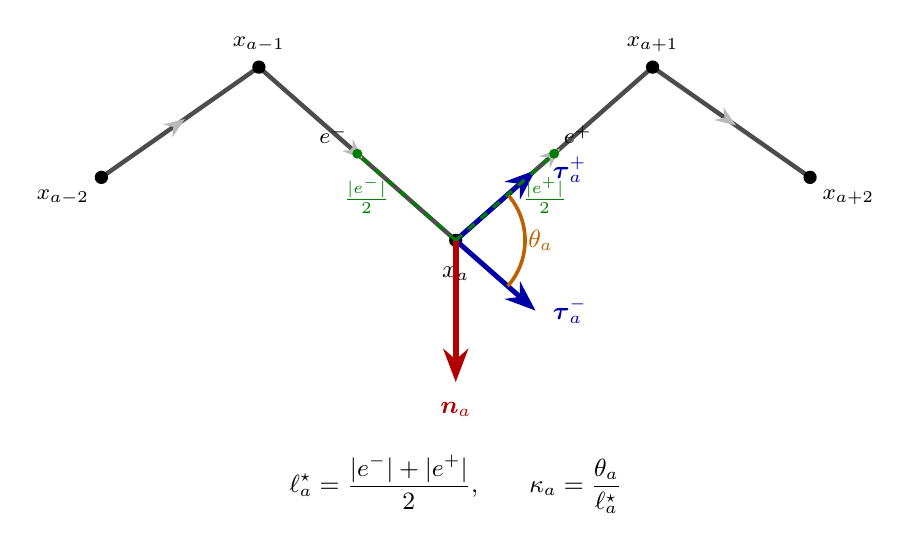
\begin{tikzpicture}[>=Stealth, font=\small]

\coordinate (Xm2) at (-4.5,  0.8);
\coordinate (Xm1) at (-2.5,  2.2);
\coordinate (Xa)  at ( 0,    0  );
\coordinate (Xp1) at ( 2.5,  2.2);
\coordinate (Xp2) at ( 4.5,  0.8);

\draw[black!70, line width=1.6pt]
  (Xm2)--(Xm1)--(Xa)--(Xp1)--(Xp2);

\foreach \s/\e in {Xm2/Xm1,Xm1/Xa,Xa/Xp1,Xp1/Xp2}
  \draw[->,gray!55,line width=1pt]
    ($(\s)!0.47!(\e)$)--($(\s)!0.53!(\e)$);

\foreach \p in {Xm2,Xm1,Xa,Xp1,Xp2}
  \fill (\p) circle (2.4pt);

\node[below left=1pt]  at (Xm2) {\footnotesize$x_{a-2}$};
\node[above=2pt]       at (Xm1) {\footnotesize$x_{a-1}$};
\node[below=6pt]       at (Xa)  {$x_a$};
\node[above=2pt]       at (Xp1) {\footnotesize$x_{a+1}$};
\node[below right=1pt] at (Xp2) {\footnotesize$x_{a+2}$};

\node[above left,  font=\footnotesize] at ($(Xm1)!.5!(Xa)$)  {$e^-$};
\node[above right, font=\footnotesize] at ($(Xa)!.5!(Xp1)$)  {$e^+$};

%-- e^- = Xa-Xm1 = (2.5,-2.2), |e^-| = sqrt(11.09) ~ 3.330
%-- tau^- = (0.751,-0.661),  angle ~ -41.3 deg
%-- tau^+ = (0.751, 0.661),  angle ~ +41.3 deg
\draw[->,blue!65!black, line width=1.8pt]
  (Xa)--++({0.751*1.35},{-0.661*1.35})
  node[right=2pt,blue!65!black]{$\boldsymbol{\tau}_a^-$};
\draw[->,blue!65!black, line width=1.8pt]
  (Xa)--++({0.751*1.35},{ 0.661*1.35})
  node[right=2pt,blue!65!black]{$\boldsymbol{\tau}_a^+$};

\draw[->,red!70!black, line width=2.0pt]
  (Xa)--++(0,-1.8)
  node[below=3pt,red!70!black]{$\boldsymbol{n}_a$};

%-- turning angle arc (CCW from tau^- to tau^+, radius 0.88)
\draw[orange!75!black, line width=1.3pt]
  ($(Xa)+({0.88*cos(-41.3)},{0.88*sin(-41.3)})$)
  arc[start angle=-41.3, end angle=41.3, radius=0.88];
\node[orange!75!black] at ($(Xa)+(1.08,0)$) {$\theta_a$};

%-- dual-length dashed marks (midpoints of e^-, e^+)
\coordinate (Mm) at (-1.25, 1.10);
\coordinate (Mp) at ( 1.25, 1.10);

\draw[green!50!black, dashed, line width=1.1pt] (Xa)--(Mm);
\draw[green!50!black, dashed, line width=1.1pt] (Xa)--(Mp);
\fill[green!50!black] (Mm) circle (1.8pt);
\fill[green!50!black] (Mp) circle (1.8pt);
\node[green!50!black, font=\footnotesize, left=2pt]
  at ($(Xa)!.52!(Mm)$) {$\tfrac{|e^-|}{2}$};
\node[green!50!black, font=\footnotesize, right=2pt]
  at ($(Xa)!.52!(Mp)$) {$\tfrac{|e^+|}{2}$};

\node[font=\small, align=center] at (0,-3.1){
  $\ell_a^\star = \dfrac{|e^-|+|e^+|}{2}$,\qquad
  $\kappa_a     = \dfrac{\theta_a}{\ell_a^\star}$};

\end{tikzpicture}

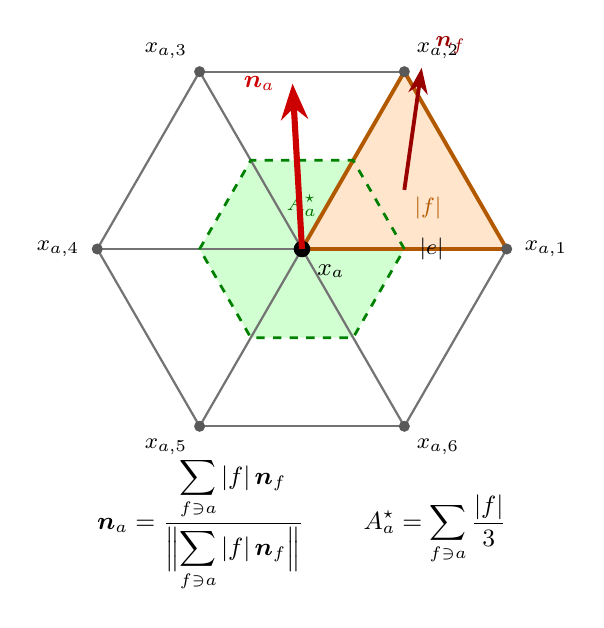
\begin{tikzpicture}[>=Stealth, font=\small]

\coordinate (Xa) at (0,     0    );
\coordinate (X1) at ( 2.6,  0    );
\coordinate (X2) at ( 1.3,  2.252);
\coordinate (X3) at (-1.3,  2.252);
\coordinate (X4) at (-2.6,  0    );
\coordinate (X5) at (-1.3, -2.252);
\coordinate (X6) at ( 1.3, -2.252);

%-- midpoint hexagon = dual area A_a*
\coordinate (M1) at ( 1.3,  0    );
\coordinate (M2) at ( 0.65, 1.126);
\coordinate (M3) at (-0.65, 1.126);
\coordinate (M4) at (-1.3,  0    );
\coordinate (M5) at (-0.65,-1.126);
\coordinate (M6) at ( 0.65,-1.126);

\fill[green!18] (M1)--(M2)--(M3)--(M4)--(M5)--(M6)--cycle;

%-- highlight face f = (Xa,X1,X2)
\fill[orange!20] (Xa)--(X1)--(X2)--cycle;

%-- all mesh edges
\foreach \r/\s in {X1/X2,X2/X3,X3/X4,X4/X5,X5/X6,X6/X1}
  \draw[black!55, line width=0.8pt] (\r)--(\s);
\foreach \r in {X1,X2,X3,X4,X5,X6}
  \draw[black!55, line width=0.8pt] (Xa)--(\r);

%-- redraw highlighted face on top
\draw[orange!70!black, line width=1.4pt] (Xa)--(X1)--(X2)--cycle;

%-- dual area border
\draw[green!50!black, dashed, line width=1.0pt]
  (M1)--(M2)--(M3)--(M4)--(M5)--(M6)--cycle;
\node[green!45!black, font=\footnotesize] at (0, 0.55) {$A_a^\star$};

%-- vertex dots
\fill[black] (Xa) circle (3pt);
\foreach \r in {X1,X2,X3,X4,X5,X6}
  \fill[black!65] (\r) circle (2pt);

%-- vertex labels
\node[below right=2pt]             at (Xa) {$x_a$};
\node[right=3pt,  font=\footnotesize] at (X1) {$x_{a,1}$};
\node[above right=1pt,font=\footnotesize] at (X2) {$x_{a,2}$};
\node[above left=1pt, font=\footnotesize] at (X3) {$x_{a,3}$};
\node[left=3pt,  font=\footnotesize]  at (X4) {$x_{a,4}$};
\node[below left=1pt, font=\footnotesize] at (X5) {$x_{a,5}$};
\node[below right=1pt,font=\footnotesize] at (X6) {$x_{a,6}$};

%-- edge and face labels
\node[right=2pt, font=\footnotesize]       at ($(Xa)!0.5!(X1)$) {$|e|$};
\node[orange!70!black, font=\footnotesize] at (1.6, 0.52)        {$|f|$};

%-- face normal n_f at centroid of highlighted face (1.3, 0.751)
\coordinate (Cf1) at (1.3, 0.751);
\draw[->, red!60!black, line width=1.4pt]
  (Cf1)--++(0.22,1.55)
  node[above right=1pt, red!60!black, font=\footnotesize]{$\boldsymbol{n}_f$};

%-- vertex normal n_a (weighted average direction, nearly vertical)
\draw[->, red!80!black, line width=2.2pt]
  (Xa)--++(-0.12, 2.1)
  node[left=2pt, red!80!black]{$\boldsymbol{n}_a$};

\node[font=\small, align=center] at (0,-3.5){
  $\boldsymbol{n}_a
   =\dfrac{\displaystyle\sum_{f\ni a}|f|\,\boldsymbol{n}_f}
          {\displaystyle\Bigl\|\sum_{f\ni a}|f|\,\boldsymbol{n}_f\Bigr\|}$
  \qquad
  $A_a^\star=\displaystyle\sum_{f\ni a}\dfrac{|f|}{3}$};

\end{tikzpicture}

\tdplotsetmaincoords{65}{20}
\begin{tikzpicture}[tdplot_main_coords, >=Stealth, font=\small, scale=1.1]

%--- Dome-shaped vertices ---
% Central vertex at apex
\coordinate (Xa) at ( 0,      0,      1.8);
% Six ring vertices (curved downward away from apex)
\coordinate (X1) at ( 2.5,    0,      0.40);
\coordinate (X2) at ( 1.25,   2.165,  0.10);
\coordinate (X3) at (-1.25,   2.165,  0.25);
\coordinate (X4) at (-2.5,    0,      0.40);
\coordinate (X5) at (-1.25,  -2.165,  0.15);
\coordinate (X6) at ( 1.25,  -2.165,  0.05);

%--- Outer partial ring for visual depth ---
\coordinate (P1) at ( 4.2,  -1.5,   -0.70);
\coordinate (P2) at ( 4.2,   1.5,   -0.70);
\coordinate (P3) at ( 2.2,   4.2,   -0.80);

%--- Dual area A_a* boundary ---
% Midpoints of spoke edges Mi = (Xa+Xi)/2
\coordinate (M1) at ( 1.250,  0.000,  1.100);
\coordinate (M2) at ( 0.625,  1.083,  0.950);
\coordinate (M3) at (-0.625,  1.083,  1.025);
\coordinate (M4) at (-1.250,  0.000,  1.100);
\coordinate (M5) at (-0.625, -1.083,  0.975);
\coordinate (M6) at ( 0.625, -1.083,  0.925);
% Face centroids Cij = (Xa+Xi+Xj)/3
\coordinate (C12) at ( 1.250,  0.722,  0.767);
\coordinate (C23) at ( 0.000,  1.443,  0.717);
\coordinate (C34) at (-1.250,  0.722,  0.817);
\coordinate (C45) at (-1.250, -0.722,  0.783);
\coordinate (C56) at ( 0.000, -1.443,  0.667);
\coordinate (C61) at ( 1.250, -0.722,  0.750);

%--- Outer faded mesh extension ---
\fill[gray!6] (X1)--(P2)--(X2)--cycle;
\fill[gray!6] (X1)--(P1)--(X6)--cycle;
\fill[gray!5] (P1)--(P2)--(X1)--cycle;

%--- Inner faces: painter order back→front
%    (dot product of face normal with view dir, ascending)
%    X3X4≈0.37, X4X5≈0.45, X5X6≈1.16, X2X3≈3.83, X6X1≈4.06, X1X2≈5.64
\fill[blue!20] (Xa)--(X3)--(X4)--cycle;   % back-left
\fill[blue!18] (Xa)--(X4)--(X5)--cycle;   % back-left
\fill[blue!12] (Xa)--(X5)--(X6)--cycle;   % front-left
\fill[blue!15] (Xa)--(X2)--(X3)--cycle;   % back-right
\fill[blue!9]  (Xa)--(X6)--(X1)--cycle;   % front-right
\fill[orange!22](Xa)--(X1)--(X2)--cycle;  % highlighted, drawn last

%--- Dual area fill and border ---
\fill[green!18, opacity=0.85]
  (M1)--(C12)--(M2)--(C23)--(M3)--(C34)--(M4)--(C45)--(M5)--(C56)--(M6)--(C61)--cycle;
\draw[green!55!black, dashed, line width=1.0pt]
  (M1)--(C12)--(M2)--(C23)--(M3)--(C34)--(M4)--(C45)--(M5)--(C56)--(M6)--(C61)--cycle;

%--- Outer mesh edges (faded) ---
\draw[gray!38, line width=0.6pt] (X1)--(P1)--(X6);
\draw[gray!38, line width=0.6pt] (X1)--(P2)--(X2);
\draw[gray!38, line width=0.6pt] (P1)--(P2);
\draw[gray!38, line width=0.6pt] (X2)--(P3)--(P2);

%--- Inner mesh edges ---
\foreach \A/\B in {X1/X2,X2/X3,X3/X4,X4/X5,X5/X6,X6/X1}
  \draw[black!55, line width=0.9pt] (\A)--(\B);
\foreach \B in {X1,X2,X3,X4,X5,X6}
  \draw[black!55, line width=0.9pt] (Xa)--(\B);

%--- Highlighted face border ---
\draw[orange!70!black, line width=1.5pt] (Xa)--(X1)--(X2)--cycle;

%--- Vertex dots ---
\fill (Xa) circle (3.0pt);
\foreach \B in {X1,X2,X3,X4,X5,X6}
  \fill[black!60] (\B) circle (2.0pt);

%--- Vertex labels ---
\node[above right=2pt]              at (Xa) {$x_a$};
\node[right=4pt, font=\footnotesize] at (X1) {$x_{a,1}$};
\node[above right=1pt,font=\footnotesize] at (X2) {$x_{a,2}$};
\node[above left=1pt, font=\footnotesize] at (X3) {$x_{a,3}$};
\node[left=4pt, font=\footnotesize]  at (X4) {$x_{a,4}$};
\node[below left=1pt, font=\footnotesize] at (X5) {$x_{a,5}$};
\node[below right=1pt,font=\footnotesize] at (X6) {$x_{a,6}$};

%--- Face normal n_f of highlighted face (Xa,X1,X2) ---
%   n_f = (X1-Xa)x(X2-Xa) / |...| ≈ (0.453, 0.374, 0.809)
%   drawn from centroid C12, scaled by 1.5
\draw[->, red!55!black, line width=1.2pt]
  (C12)--++(0.68, 0.56, 1.21)
  node[right=3pt,font=\footnotesize,red!55!black]{$\boldsymbol{n}_f$};

%--- Vertex normal n_a at dome apex: points straight up ---
\draw[->, red!85!black, line width=2.2pt]
  (Xa)--++(0, 0, 2.3)
  node[above=2pt, red!85!black]{$\boldsymbol{n}_a$};

%--- Internal labels ---
\node[green!50!black, font=\footnotesize] at (0.1,  0.25, 1.26) {$A_a^\star$};
\node[orange!70!black,font=\footnotesize] at (1.45, 0.75, 0.63) {$|f|$};
\node[black!55,       font=\footnotesize] at (1.78, 0,    1.0 ) {$|e|$};

%--- Formula below (2D screen space, outside the 3D scope) ---
\node[font=\small, align=center, below=8pt]
  at (current bounding box.south){%
  $\boldsymbol{n}_a
   =\dfrac{\displaystyle\sum_{f\ni a}|f|\,\boldsymbol{n}_f}
          {\displaystyle\Bigl\|\sum_{f\ni a}|f|\,\boldsymbol{n}_f\Bigr\|}$
  \qquad
  $A_a^\star=\displaystyle\sum_{f\ni a}\dfrac{|f|}{3}$%
};

\end{tikzpicture}


Starting from the embedded front mesh, one reconstructs the minimal set of
metric quantities needed to define intrinsic operators.

\subsubsection{Polygonal curves in two dimensions}

Let $e=(i,j)\in E_h$ be an oriented edge of the polygonal curve.
Its length and unit tangent are
\begin{equation}
|e| = \|x_j-x_i\|,
\qquad
\tau_e = \frac{x_j-x_i}{|e|}.
\label{eq:curve_edge_data}
\end{equation}

At each vertex $x_a$, we define the dual vertex length
\begin{equation}
\ell_a^\star
=
\frac12 \sum_{e\ni a} |e|,
\label{eq:curve_dual_length}
\end{equation}
that is, half the sum of the lengths of the edges incident to that vertex.
This quantity plays the role of a vertex-based measure along the discrete curve.

The minimal metric data carried by a polygonal front are therefore
\begin{equation}
\mathcal{G}_h^{\mathrm{curve}}
=
\left\{
|e|,\ \tau_e,\ \ell_a^\star
\right\}.
\label{eq:curve_metric_tuple}
\end{equation}

\subsubsection{Triangulated surfaces in three dimensions}

Let $f=(i,j,k)\in F_h$ be an oriented triangular face.
Its non-normalized normal vector is
\begin{equation}
\widetilde{n}_f = (x_j-x_i)\times(x_k-x_i),
\label{eq:unnormalized_face_normal}
\end{equation}
and its unit normal and area are
\begin{equation}
n_f = \frac{\widetilde{n}_f}{\|\widetilde{n}_f\|},
\qquad
|f| = \frac12 \|\widetilde{n}_f\|.
\label{eq:face_area_normal}
\end{equation}

For each edge $e=(i,j)$, the edge length is
\begin{equation}
|e| = \|x_j-x_i\|.
\label{eq:surface_edge_length}
\end{equation}

At each vertex $x_a$, one defines a dual vertex area $A_a^\star$.
A simple choice is the barycentric dual area
\begin{equation}
A_a^\star
=
\sum_{f\ni a}\frac{|f|}{3},
\label{eq:barycentric_dual_area}
\end{equation}
obtained by assigning one third of each incident triangle area to each of its vertices.
More elaborate mixed dual areas may also be used, but the present notation remains unchanged.

The minimal metric data carried by a triangulated front are therefore
\begin{equation}
\mathcal{G}_h^{\mathrm{surf}}
=
\left\{
|e|,\ |f|,\ A_a^\star,\ n_f,\ \omega_e
\right\},
\label{eq:surface_metric_tuple}
\end{equation}
where $\omega_e$ denotes the edge-based metric coefficient entering the discrete
Hodge star on tangential $1$-forms. For the standard cotangent Laplace--Beltrami
operator on a triangulated surface, $\omega_e$ is the usual cotangent weight
associated with the edge $e$.

\subsection{Dual measures and Hodge stars}
\label{subsec:front_hodge}

The incidence operators defined above are purely combinatorial.
Metric information enters through discrete Hodge stars, which weight primal
cochains by the appropriate dual measures.

For a polygonal curve, the vertex Hodge star is
\begin{equation}
\star_0 = \operatorname{diag}\!\left(\ell_1^\star,\ldots,\ell_{N_v}^\star\right),
\label{eq:hodge0_curve}
\end{equation}
while the edge Hodge star is
\begin{equation}
\star_1 = \operatorname{diag}\!\left(|e_1|^{-1},\ldots,|e_{N_e}|^{-1}\right).
\label{eq:hodge1_curve}
\end{equation}

For a triangulated surface, the vertex Hodge star is
\begin{equation}
\star_0 = \operatorname{diag}\!\left(A_1^\star,\ldots,A_{N_v}^\star\right),
\label{eq:hodge0_surface}
\end{equation}
and the edge Hodge star is
\begin{equation}
\star_1 = \operatorname{diag}\!\left(\omega_{e_1},\ldots,\omega_{e_{N_e}}\right),
\label{eq:hodge1_surface}
\end{equation}
where $\omega_e$ denotes the edge-based metric coefficient associated with the
discrete tangential $1$-form on edge $e$. In the standard cotangent formulation,
$\omega_e$ is the usual cotangent weight.

If face-based $2$-cochains are needed, the face Hodge star is
\begin{equation}
\star_2 = \operatorname{diag}\!\left(|f_1|,\ldots,|f_{N_f}|\right).
\label{eq:hodge2_surface}
\end{equation}

These Hodge stars provide the metric structure required to define intrinsic
differential operators on the front.

\subsection{Intrinsic differential operators on the front}
\label{subsec:front_operators}

\subsubsection{Tangential projection}

Let $n$ denote a unit normal field on the front.
For any ambient vector $v\in\mathbb{R}^d$, its tangential projection onto the
local tangent space of the interface is
\begin{equation}
\Pi_\Gamma(v) = v - (v\cdot n)n.
\label{eq:tangential_projection}
\end{equation}
This decomposition separates normal motion of the interface from tangential
redistribution along the front.

\subsubsection{Laplace-Beltrami operator}

Let $u_h\in C^0(\Gamma_h)$ be a scalar field defined at the front vertices.
Its intrinsic Laplace-Beltrami operator is written in discrete exterior calculus form as
\begin{equation}
\Delta_{\Gamma_h} u_h
=
\star_0^{-1} d_0^\top \star_1 d_0 u_h.
\label{eq:laplace_beltrami}
\end{equation}
This formula applies both to polygonal curves and triangulated surfaces, provided
the edge Hodge star $\star_1$ is chosen consistently with the underlying metric.
For a curve, \eqref{eq:laplace_beltrami} approximates the second derivative along arclength.
For a triangulated surface, it yields the standard edge-weighted discrete surface
Laplacian, including the cotangent form as a particular case.
The operator is intrinsic in the sense that it depends only on the metric and
topology of the front mesh.

\subsubsection{Surface gradient on a triangulated surface}

When $d=3$, a scalar field $u_h=\{u_a\}_{a=1}^{N_v}$ defined at the vertices of a
triangulated surface induces a piecewise constant tangential gradient on each face.
For a face $f=(a,b,c)$, one has
\begin{equation}
\nabla_{\Gamma_h} u_h \big|_f
=
\frac{1}{2|f|}
\left[
u_a\, n_f\times(x_c-x_b)
+
u_b\, n_f\times(x_a-x_c)
+
u_c\, n_f\times(x_b-x_a)
\right].
\label{eq:surface_gradient}
\end{equation}
This expression is exact for piecewise affine scalar fields on the triangulation.

Together, the tangential projection, the Laplace-Beltrami operator, and the
surface gradient provide the core intrinsic differential tools needed later for the front evolution equations.


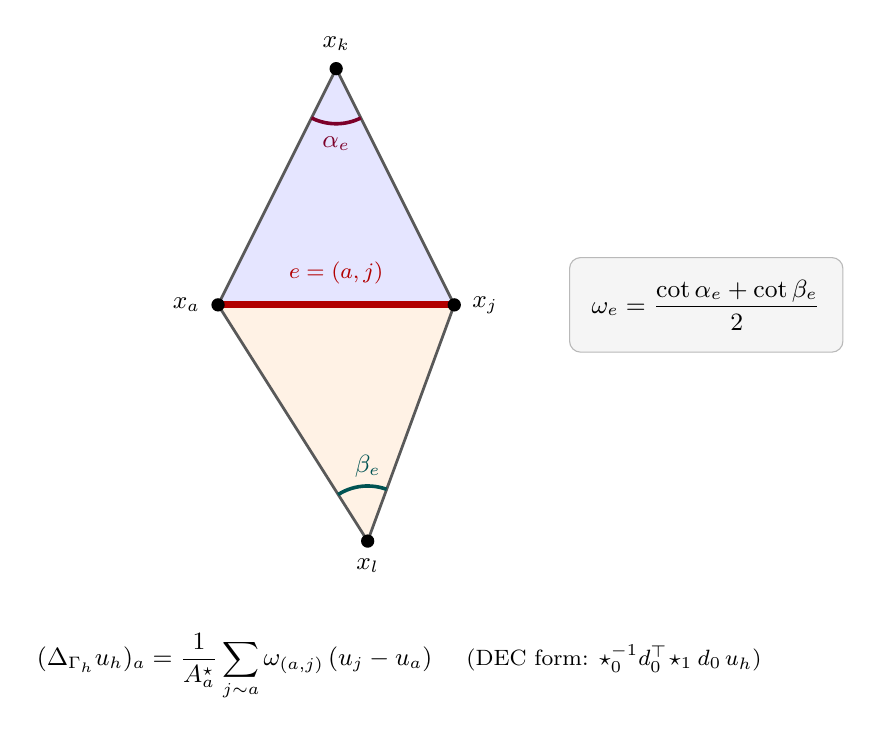
\begin{tikzpicture}[>=Stealth, font=\small]

\coordinate (Xa) at (-1.5,  0);
\coordinate (Xj) at ( 1.5,  0);
\coordinate (Xk) at ( 0,    3);
\coordinate (Xl) at ( 0.4, -3);

\fill[blue!10]   (Xa)--(Xj)--(Xk)--cycle;
\fill[orange!10] (Xa)--(Xj)--(Xl)--cycle;

\draw[black!65, line width=1.0pt] (Xa)--(Xj)--(Xk)--cycle;
\draw[black!65, line width=1.0pt] (Xa)--(Xj)--(Xl)--cycle;

%-- highlighted edge
\draw[red!70!black, line width=2.5pt] (Xa)--(Xj);
\node[above=4pt, red!70!black, font=\footnotesize] at (0,0) {$e=(a,j)$};

\foreach \p in {Xa,Xj,Xk,Xl}
  \fill (\p) circle (2.4pt);

\node[left=3pt]  at (Xa) {$x_a$};
\node[right=3pt] at (Xj) {$x_j$};
\node[above=3pt] at (Xk) {$x_k$};
\node[below=3pt] at (Xl) {$x_l$};

%-- angle alpha_e at Xk
%   Xk=(0,3): to Xa angle=243.43 deg, to Xj angle=296.57 deg
\draw[purple!65!black, line width=1.3pt]
  ($(Xk)+({0.7*cos(243.43)},{0.7*sin(243.43)})$)
  arc[start angle=243.43, end angle=296.57, radius=0.7];
\node[purple!65!black] at ($(Xk)+(0,-0.95)$) {$\alpha_e$};

%-- angle beta_e at Xl
%   Xl=(0.4,-3): to Xa angle=122.41 deg, to Xj angle=69.87 deg
\draw[teal!65!black, line width=1.3pt]
  ($(Xl)+({0.7*cos(69.87)},{0.7*sin(69.87)})$)
  arc[start angle=69.87, end angle=122.41, radius=0.7];
\node[teal!65!black] at ($(Xl)+(0,0.95)$) {$\beta_e$};

%-- cotangent weight box
\node[draw=gray!55, fill=gray!8, rounded corners=4pt,
      font=\small, inner sep=8pt]
  at (4.7, 0){
    $\omega_e = \dfrac{\cot\alpha_e+\cot\beta_e}{2}$};

%-- Laplace--Beltrami formula
\node[font=\small, align=center] at (0.8,-4.6){
  $(\Delta_{\Gamma_h} u_h)_a
   =\dfrac{1}{A_a^\star}
    \displaystyle\sum_{j\sim a}\omega_{(a,j)}\,(u_j-u_a)$
  \quad\footnotesize(DEC form: $\star_0^{-1}d_0^\top\!\star_1 d_0\, u_h$)};

\end{tikzpicture}

\subsection{Normals and curvature}
\label{subsec:front_curvature}

We now introduce the geometric quantities derived from the front representation.

\subsubsection{Normals and curvature of a polygonal curve}

Let $x_a$ be a vertex of the polygonal curve, and let $\tau_a^-$ and $\tau_a^+$ denote
the incoming and outgoing unit tangents of the incident edges.
A discrete vertex tangent is obtained from their normalized average, and the
corresponding unit normal $n_a$ is obtained by a quarter-turn rotation in the plane.
The choice of rotation sign is fixed globally so as to remain consistent with
the interface normal convention of Section~\ref{sec:governing}.

The discrete signed curvature at vertex $x_a$ is defined by
\begin{equation}
\kappa_a
=
\frac{\theta_a}{\ell_a^\star},
\label{eq:curve_curvature}
\end{equation}
where $\theta_a$ is the signed turning angle from $\tau_a^-$ to $\tau_a^+$ and
$\ell_a^\star$ is the dual vertex length defined in \eqref{eq:curve_dual_length}.
This quantity converges to the continuous signed curvature as the polygonal front is refined.

\subsubsection{Normals and curvature of a triangulated surface}

For a triangulated surface, the face normals $n_f$ are already defined in
\eqref{eq:face_area_normal}. A vertex normal is obtained by averaging the normals
of the incident faces with area weights,
\begin{equation}
n_a
=
\frac{
\sum\limits_{f\ni a} |f|\,n_f
}{
\left\|
\sum\limits_{f\ni a} |f|\,n_f
\right\|
}.
\label{eq:vertex_normal_surface}
\end{equation}

The discrete mean-curvature normal is then defined from the Laplace--Beltrami
operator applied componentwise to the embedding $X=\{x_a\}_{a=1}^{N_v}$:
\begin{equation}
\boldsymbol{H}_a
=
-\frac12\left(\Delta_{\Gamma_h} X\right)_a.
\label{eq:mean_curvature_vector}
\end{equation}
Its scalar projection on the vertex normal gives the discrete mean curvature,
\begin{equation}
H_a = \boldsymbol{H}_a \cdot n_a.
\label{eq:mean_curvature_scalar}
\end{equation}
This convention is consistent with the continuous identity
$\Delta_\Gamma X = -2H n$. If one uses the twice-mean-curvature convention
$\kappa=2H$, then the corresponding curvature normal is
$\boldsymbol{\kappa}_a=2\boldsymbol{H}_a$.

The Gaussian curvature is defined through the angle defect formula
\begin{equation}
K_a
=
\frac{1}{A_a^\star}
\left(
2\pi - \sum_{f\ni a}\theta_a^f
\right),
\label{eq:gaussian_curvature}
\end{equation}
where $\theta_a^f$ denotes the interior angle of face $f$ at vertex $x_a$.
The quantities $n_a$, $H_a$, and $K_a$ form the minimal curvature data attached
to a triangulated surface front.

\subsection{Global geometric diagnostics}
\label{subsec:front_diagnostics}

The front representation also provides global geometric quantities that are useful
for verification and monitoring.

\paragraph{Front measure.}
For a polygonal curve, the total front length is
\begin{equation}
|\Gamma_h| = \sum_{e\in E_h} |e|,
\label{eq:front_length}
\end{equation}
whereas for a triangulated surface, the total front area is
\begin{equation}
|\Gamma_h| = \sum_{f\in F_h} |f|.
\label{eq:front_area}
\end{equation}

\paragraph{Enclosed measure.}
If the front is closed, it also defines an enclosed geometric measure:
an enclosed area in two dimensions and an enclosed volume in three dimensions.


\paragraph{Topological diagnostics.}
For a closed triangulated surface, the Euler characteristic is
\begin{equation}
\chi = N_v - N_e + N_f,
\label{eq:euler_characteristic}
\end{equation}
where $N_e$ is the number of unique edges.
Combined with the discrete Gaussian curvature, it yields the Gauss-Bonnet relation
\begin{equation}
\sum_{a=1}^{N_v} K_a A_a^\star = 2\pi \chi,
\label{eq:gauss_bonnet}
\end{equation}
for a closed triangulated surface without boundary, up to floating-point roundoff.
This identity is a useful diagnostic for curvature consistency and mesh integrity.

The front-based quantities introduced above are intrinsic to the Lagrangian mesh. 



\bibliographystyle{plain}
\bibliography{references}

\end{document}
